\documentclass{standalone}
\usepackage[utf8]{inputenc}
\usepackage[T1]{fontenc}
\usepackage{ngerman}
\usepackage{xcolor}
\usepackage{fixltx2e}
\usepackage{tikz}
\usepackage{titlesec}
\usepackage{booktabs}

\usetikzlibrary{shapes,positioning,arrows,backgrounds,calc,fit}
%\usetikzlibrary{shapes.geometric,backgrounds,positioning-plus,node-families,calc}
%\usetikzlibrary{shapes.geometric,backgrounds,calc}

% http://www.texample.net/tikz/examples/flowchart/

\definecolor{fhgg}{RGB}{23,156,125} % green
\definecolor{fhgo}{RGB}{235,106,10} % orange
\definecolor{fhgdb}{RGB}{0,110,146} % dark blue
\definecolor{fhglb}{RGB}{37,186,226} % light blue
\definecolor{fhgy}{RGB}{177,200,0} % yellow green

\newcommand{\cfile}{fhglb!20!white}
\newcommand{\csel}{fhgo!20!white}
\newcommand{\cbuf}{fhgg!20!white}
\newcommand{\calg}{fhgy!20!white}

\tikzset{
	every node/.style = { align = center, draw },
	io/.style = { signal, signal to=south, signal pointer angle=150, fill=\cfile, minimum width=20mm },
	alg/.style = { rectangle, minimum width=15mm, minimum height=6mm, fill=\calg },
	clr/.style = { draw=none },
	head/.style = { clr, font=\large },
	buf/.style = { cylinder, shape aspect=.5, fill=\cbuf },
	op/.style = { circle, fill=\calg },
 	cfg/.style = { buf, font=\scriptsize },
	dsc/.style = { clr, font=\scriptsize, align=left, anchor=west },
	blk/.style = { inner sep=3mm, color=fhgdb, append after command={
		\pgfextra{\let\TikZlastnode\tikzlastnode}
		node [draw=none,anchor=north west,text=fhgdb] (blk-\TikZlastnode) at (\TikZlastnode.north west) {#1}
	}},
}



\begin{document}
\pagestyle{empty}
\thispagestyle{empty}
\sffamily

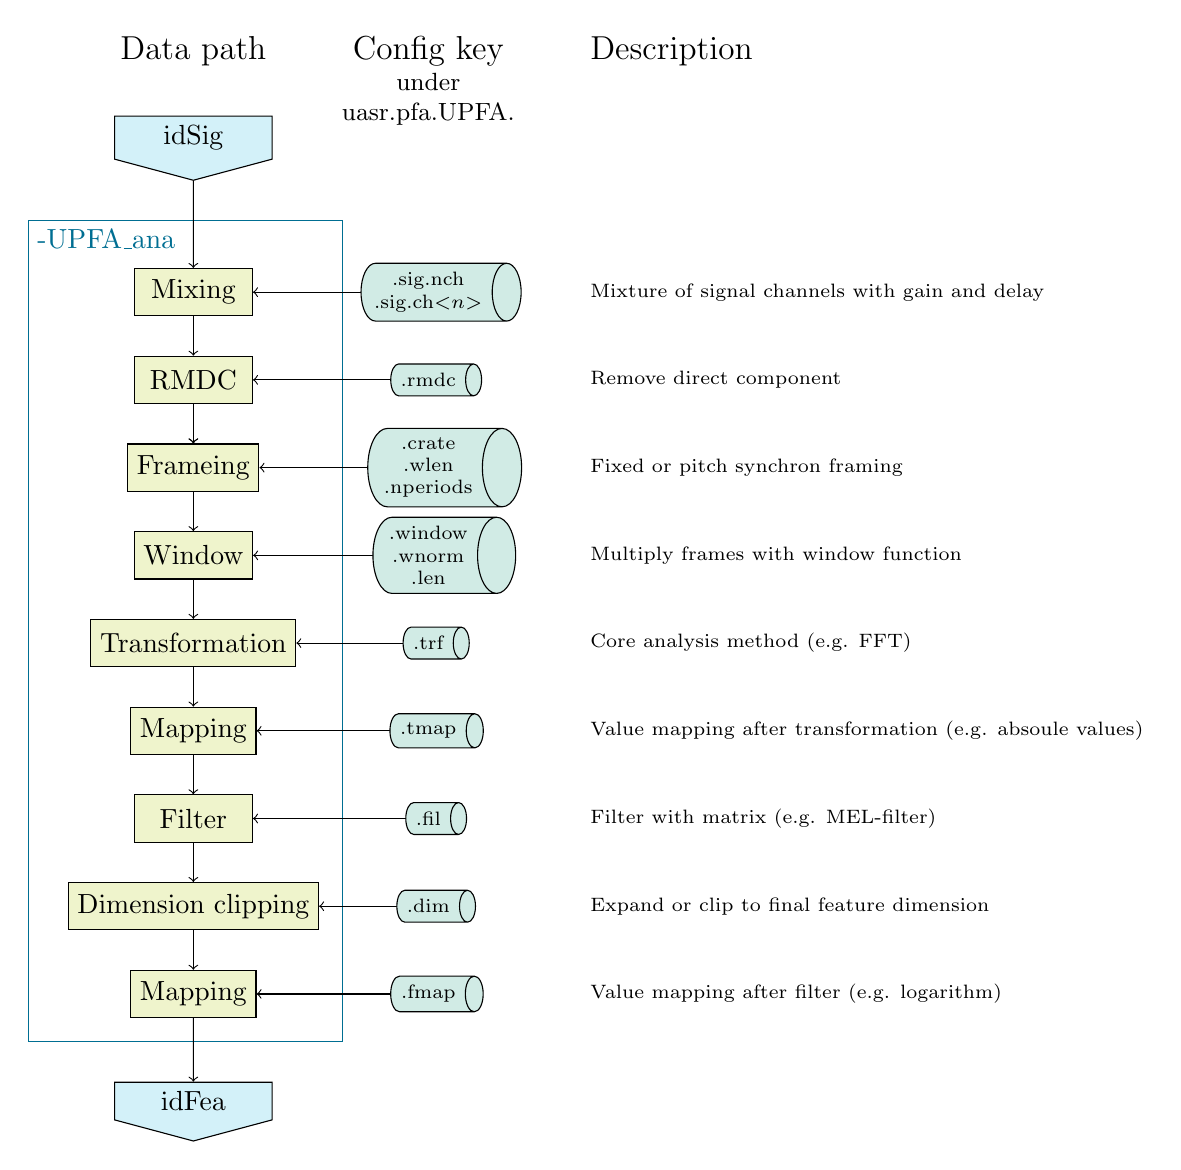
\begin{tikzpicture}[node distance=5mm]
\node (mix)   [alg]               {Mixing};
\node (rmdc)  [alg,below=of mix]  {RMDC};
\node (frm)   [alg,below=of rmdc] {Frameing};
\node (wnd)   [alg,below=of frm]  {Window};
\node (trf)   [alg,below=of wnd]  {Transformation};
\node (tmap)  [alg,below=of trf]  {Mapping};
\node (fil)   [alg,below=of tmap] {Filter};
\node (dim)   [alg,below=of fil]  {Dimension clipping};
\node (fmap)  [alg,below=of dim]  {Mapping};
\draw[->] (mix)  -- (rmdc);
\draw[->] (rmdc) -- (frm);
\draw[->] (rmdc) -- (frm);
\draw[->] (frm)  -- (wnd);
\draw[->] (wnd)  -- (trf);
\draw[->] (trf)  -- (tmap);
\draw[->] (tmap) -- (fil);
\draw[->] (fil)  -- (dim);
\draw[->] (dim)  -- (fmap);

\coordinate (anat) at ($(mix.north)+(0,3mm)$);
\coordinate (anal) at ($(dim.west)-(2mm,0)$);
\node (ana) [blk=-UPFA\_ana,fit=(mix)(fmap)(dim)(anal)(anat)] {};

\node (sig)   [io,above=of mix|-ana.north]   {idSig};
\node (fea)   [io,below=of fmap|-ana.south]  {idFea};  
\draw[->] (sig)  -- (mix);
\draw[->] (fmap) -- (fea);

\node (phead) [head,above=of sig] {Data path};
\node (chead) [head,right=of phead.north east,anchor=north west] {Config key \\ \small \begin{tabular}{c}under \\ uasr.pfa.UPFA.\end{tabular}};
\node (dhead) [head,right=of chead.north east,anchor=north west] {Description};

\draw[<-] (mix)  -- (chead|-mix)  node[cfg]{.sig.nch \\ .sig.ch$<$$n$$>$};
\draw[<-] (rmdc) -- (chead|-rmdc) node[cfg]{.rmdc};
\draw[<-] (frm)  -- (chead|-frm)  node[cfg]{.crate \\ .wlen \\ .nperiods};
\draw[<-] (wnd)  -- (chead|-wnd)  node[cfg]{.window \\ .wnorm \\ .len};
\draw[<-] (trf)  -- (chead|-trf)  node[cfg]{.trf};
\draw[<-] (tmap) -- (chead|-tmap) node[cfg]{.tmap};
\draw[<-] (fil)  -- (chead|-fil)  node[cfg]{.fil};
\draw[<-] (dim)  -- (chead|-dim)  node[cfg]{.dim};
\draw[<-] (fmap) -- (chead|-fmap) node[cfg]{.fmap};

\node (dmix)  [dsc] at (dhead.west|-mix)  {Mixture of signal channels with gain and delay};
\node (drmdc) [dsc] at (dhead.west|-rmdc) {Remove direct component};
\node (dfrm)  [dsc] at (dhead.west|-frm)  {Fixed or pitch synchron framing};
\node (dwnd)  [dsc] at (dhead.west|-wnd)  {Multiply frames with window function};
\node (dtrf)  [dsc] at (dhead.west|-trf)  {Core analysis method (e.g. FFT)};
\node (dtmap) [dsc] at (dhead.west|-tmap) {Value mapping after transformation (e.g. absoule values)};
\node (dfil)  [dsc] at (dhead.west|-fil)  {Filter with matrix (e.g. MEL-filter)};
\node (ddim)  [dsc] at (dhead.west|-dim)  {Expand or clip to final feature dimension};
\node (dfmap) [dsc] at (dhead.west|-fmap) {Value mapping after filter (e.g. logarithm)};

\end{tikzpicture}

\end{document}
